% https://www.overleaf.com/learn/latex/Beamer#Introduction
% https://en.wikibooks.org/wiki/LaTeX/Presentations#The_Beamer_package
\documentclass{beamer}
\usepackage[utf8]{inputenc}
% http://texblog.net/latex-archive/latex-general/beamer-warnings/
\usepackage{lmodern}
% https://hartwork.org/beamer-theme-matrix/
% \usecolortheme{dove}

\beamertemplatenavigationsymbolsempty
% https://tex.stackexchange.com/a/74251
\setbeamerfont{page number in head/foot}{size=\small}
\setbeamertemplate{footline}[frame number]
 
\author{Russel Shawn Dsouza}
% https://tex.stackexchange.com/a/61053
\institute
{
  
\includegraphics[scale=0.25]{images/logo}\\
  Electronics and Communications Engg.\\
  National Institute of Technology Karnataka\\
  Surathkal, India - 575025
}
\date{October 9, 2019}

\title[Neural TTS]{Neural Text-to-Speech}
% \subtitle{A short story}
 
\begin{document}

  % https://stackoverflow.com/a/54916411
  \begingroup
    \setbeamertemplate{footline}{}
    \frame{\titlepage}
  \endgroup

  \addtocounter{framenumber}{-1}

  % https://tex.stackexchange.com/a/198102
  % \begin{frame}{Overview}
  %   \tableofcontents
  % \end{frame}

  \begin{frame}
    \frametitle{Speech synthesis}
      Artificial production of human speech
      \begin{figure}
        \centering
        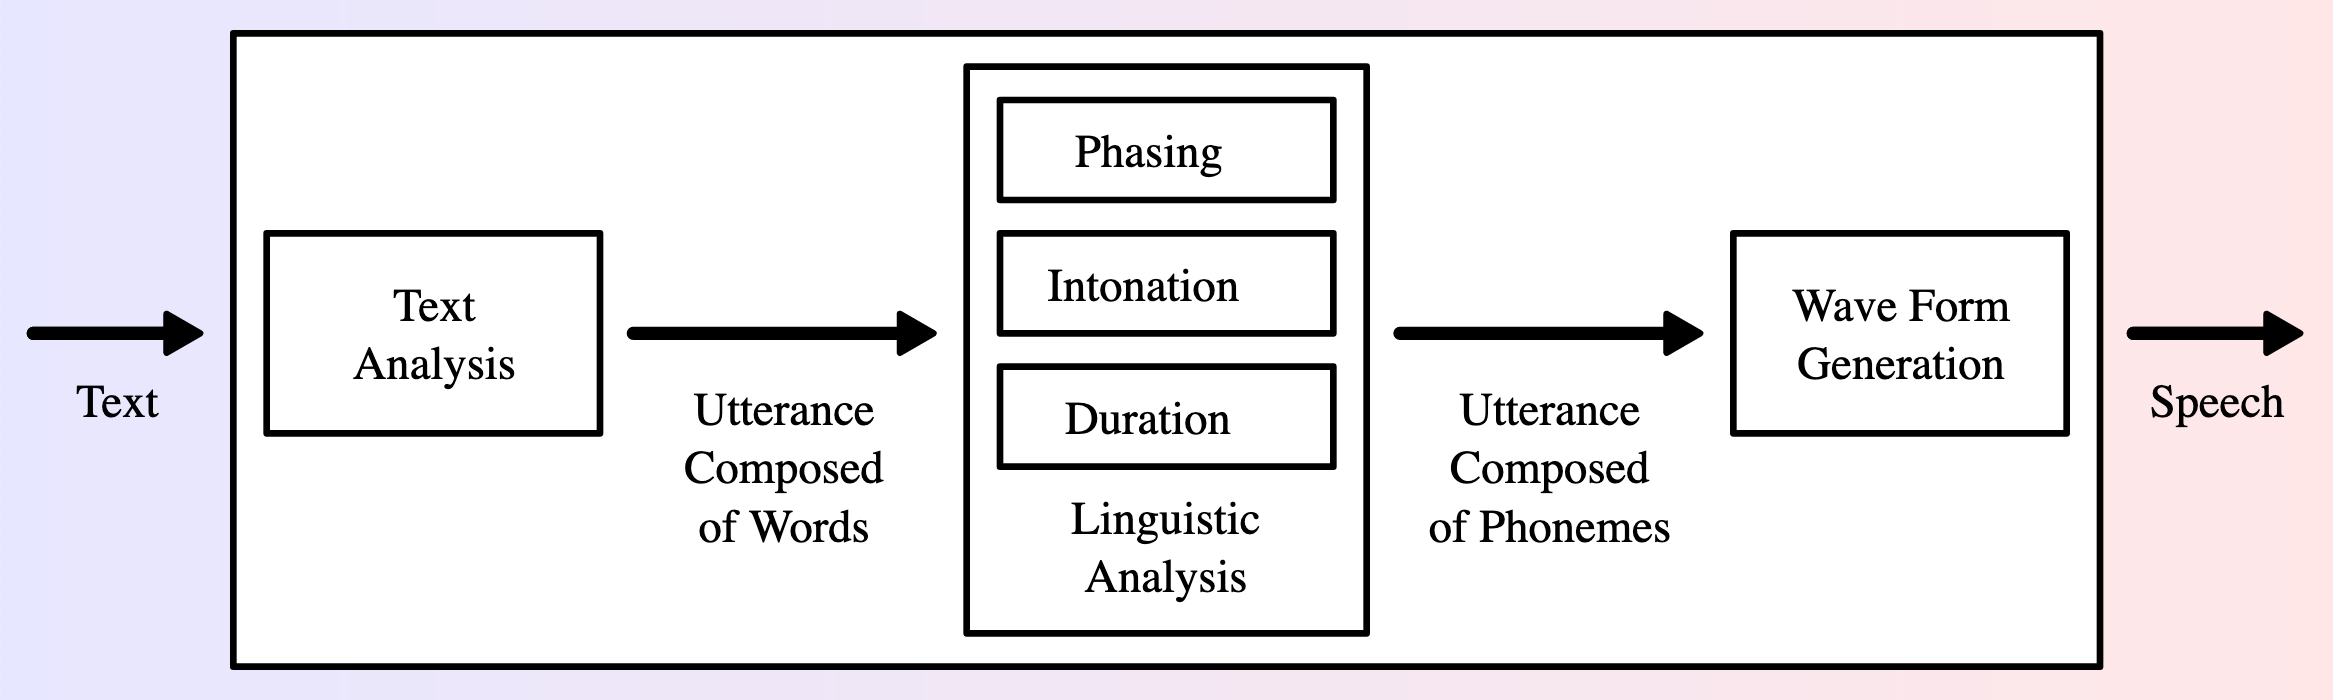
\includegraphics[width=\textwidth]{images/TTS_System_screenshot}
        \caption{A typical text-to-speech system}
      \end{figure}
  \end{frame}

  \begin{frame}
    \frametitle{History of speech synthesis}
    % TODO: Add images for each type
      \begin{columns}
        \column{0.33\textwidth}
          Concatenative
        \column{0.33\textwidth}
          Parametric
        \column{0.33\textwidth}
          Neural
      \end{columns}
  \end{frame}

  \begin{frame}
    \frametitle{Approaches in Neural text-to-speech}
      % TODO: Add images for each type
      \begin{columns}
        \column{0.33\textwidth}
          LSTM
        \column{0.33\textwidth}
          WaveNet
        \column{0.33\textwidth}
          WaveNet based
      \end{columns}
  \end{frame}

  \begin{frame}
    \frametitle{WaveNet}
      A deep neural network for generating raw audiowaveforms.

      \begin{itemize}
        \item Probabilistic 
        \item Autoregressive
        \item Beats all previously known methods
      \end{itemize}
      \begin{figure}
        \centering
        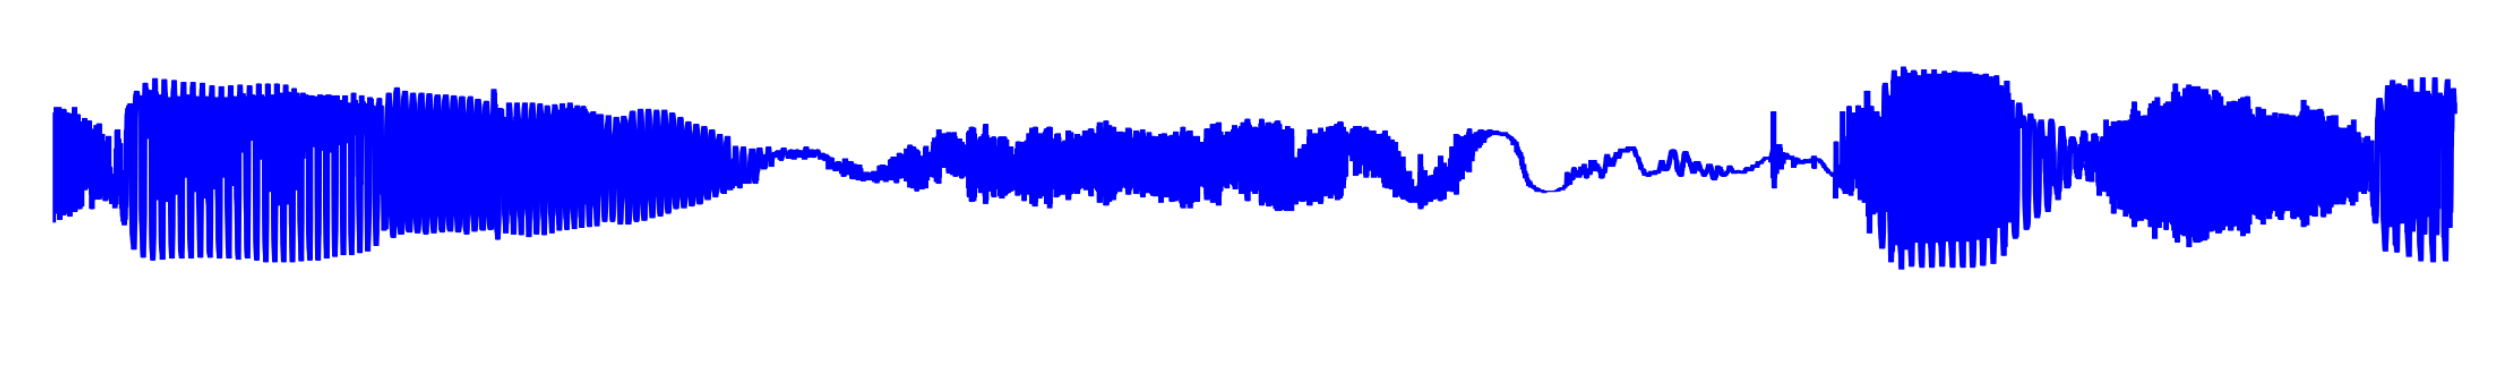
\includegraphics[width=\textwidth]{images/second_of_speech.png}
        \caption{Time domain representation of 1 second of generated speech}
      \end{figure}
  \end{frame}

  \begin{frame}
    \frametitle{WaveNet: Architecture}
  \end{frame}

  \begin{frame}
    \frametitle{WaveNet: Pros and Cons}
  \end{frame}

  \begin{frame}
    \frametitle{FloWaveNet}

  \end{frame}

  \begin{frame}
    \frametitle{FloWaveNet: Architecture}
  \end{frame}

  \begin{frame}
    \frametitle{FloWaveNet: Training}
  \end{frame}

  \begin{frame}
    \frametitle{FloWaveNet: Reported results}
  \end{frame}

  \begin{frame}
    \frametitle{FloWaveNet: Improvements over WaveNet}
  \end{frame}

  \begin{frame}
    \frametitle{Neural TTS: The future}
  \end{frame}

  \begin{frame}
    \frametitle{Summary}
  \end{frame}

  \begin{frame}
    \frametitle{Conclusion}
  \end{frame}
  
\end{document}
